\fbckg{background/mathematics_model}
\begin{frame}
    \Huge
    \misc{Modelos de transferencia radiativa}
\end{frame}

\fbckg{background/white}
\begin{frame}
    \misc{
        \begin{minipage}{0.42\linewidth}
            \begin{figure}[H]
                \centering
                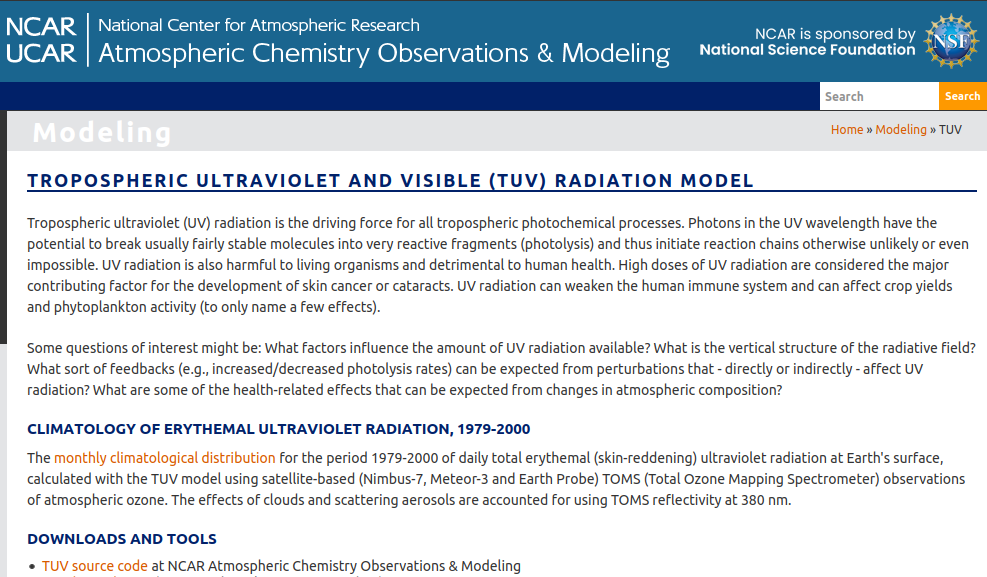
\includegraphics[height=4cm,width=5.5cm]{tuv_model.png}
                \caption{Tropospheric Ultraviolet and Visible (TUV) radiation model. \cite{tuv_model_page}}
            \end{figure}
        \end{minipage}
        \hspace{1cm}
        \begin{minipage}{0.49\linewidth}
            \begin{figure}[H]
                \centering
                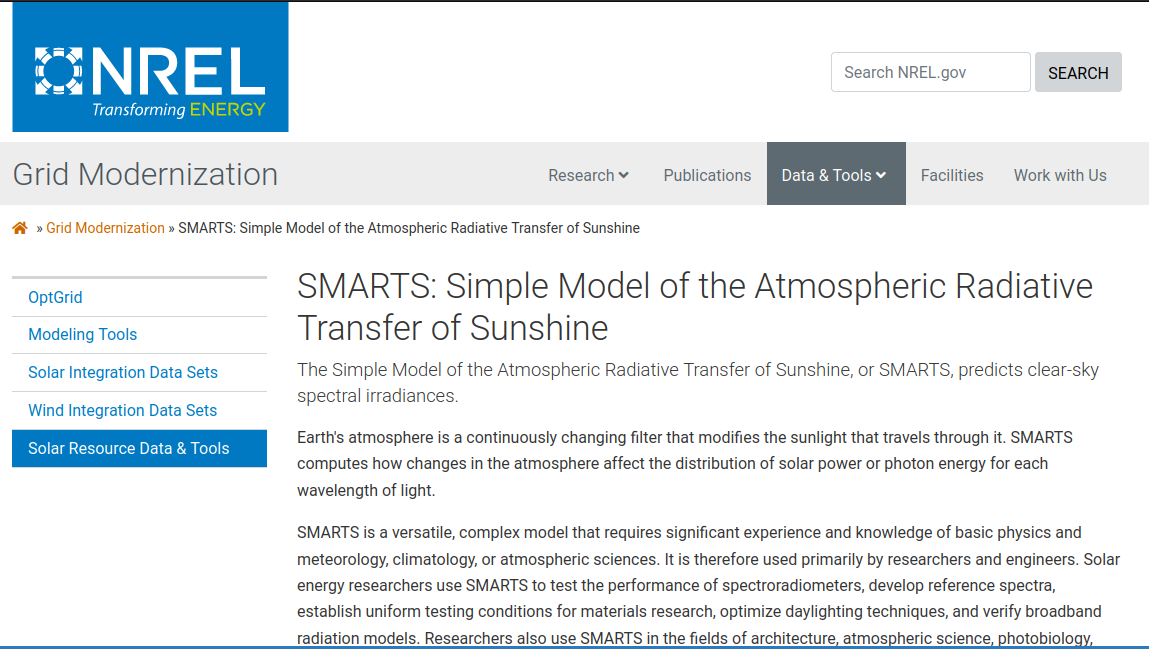
\includegraphics[height=4cm,width=5.5cm]{smarts_model.png}
                \caption{Simple Model of the Atmospheric Radiative Transfer of Sunshine. \cite{SMARTS_model_page}}
            \end{figure}
        \end{minipage}}
\end{frame}

\begin{frame}
    \misc{
        \Huge
        ¿Qué hacen estos modelos?
    }
\end{frame}

\begin{frame}
    \misc{
        \Huge
        \begin{equation*}
            \frac{d E }{dA dt} = I_\nu(\hat{k},\vec{r},t)\vec{k} \cdot \vec{n} d\Omega d\nu \qquad \cite{Carrami_2020}
        \end{equation*}
    }
\end{frame}

\begin{frame}
    \renewcommand{\yourowntexcol}{black}
    \begin{minipage}{0.40\linewidth}
        \begin{figure}[H]
            \centering
            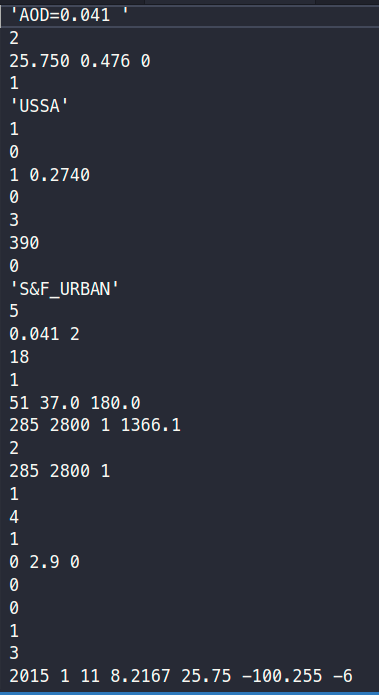
\includegraphics[width=4cm]{SMARTS_input.png}
            \caption{Archivo de inputs del modelo SMARTS}
        \end{figure}
    \end{minipage}
    \begin{minipage}{0.55\linewidth}
        \begin{figure}[H]
            \centering
            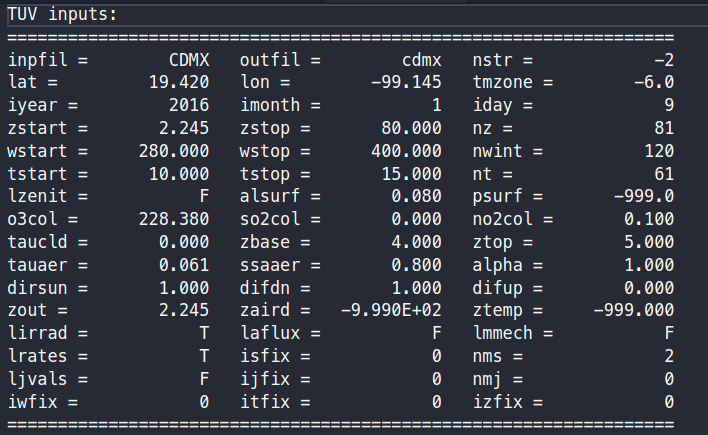
\includegraphics[width=8cm]{tuv_input.png}
            \caption{Archivo de inputs del modelo TUV}
        \end{figure}
    \end{minipage}
\end{frame}

\begin{frame}
    \misc{
        \Huge
        \begin{equation}
            I(t) = \int\limits_{\lambda_0}^{\lambda_i} E(\lambda, t) d\lambda
            \label{eq:integral}
        \end{equation}
    }
\end{frame}

\begin{frame}
    \misc{
        \begin{figure}
            \centering
            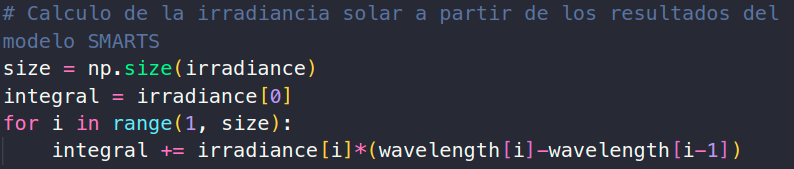
\includegraphics[width=11cm]{code_integral.png}
            \caption{Implementación de la ecuación \ref{eq:integral}.}
        \end{figure}
    }
\end{frame}

\begin{frame}
    \hspace{-0.75cm}
    \begin{minipage}{0.45\linewidth}
        \begin{figure}[H]
            \color{black}
            \centering
            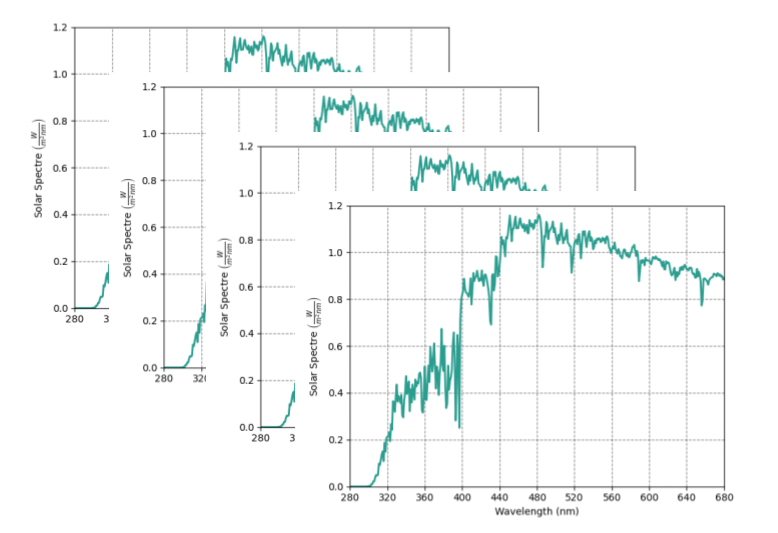
\includegraphics[width=7cm]{spectre.png}
        \end{figure}
    \end{minipage}
    \hspace{0.5cm}
    \begin{minipage}{0.12\linewidth}
        \Huge
        \begin{equation*}
            \color{black}
            \rightarrow
        \end{equation*}
    \end{minipage}
    \begin{minipage}{0.38\linewidth}
        \begin{figure}[H]
            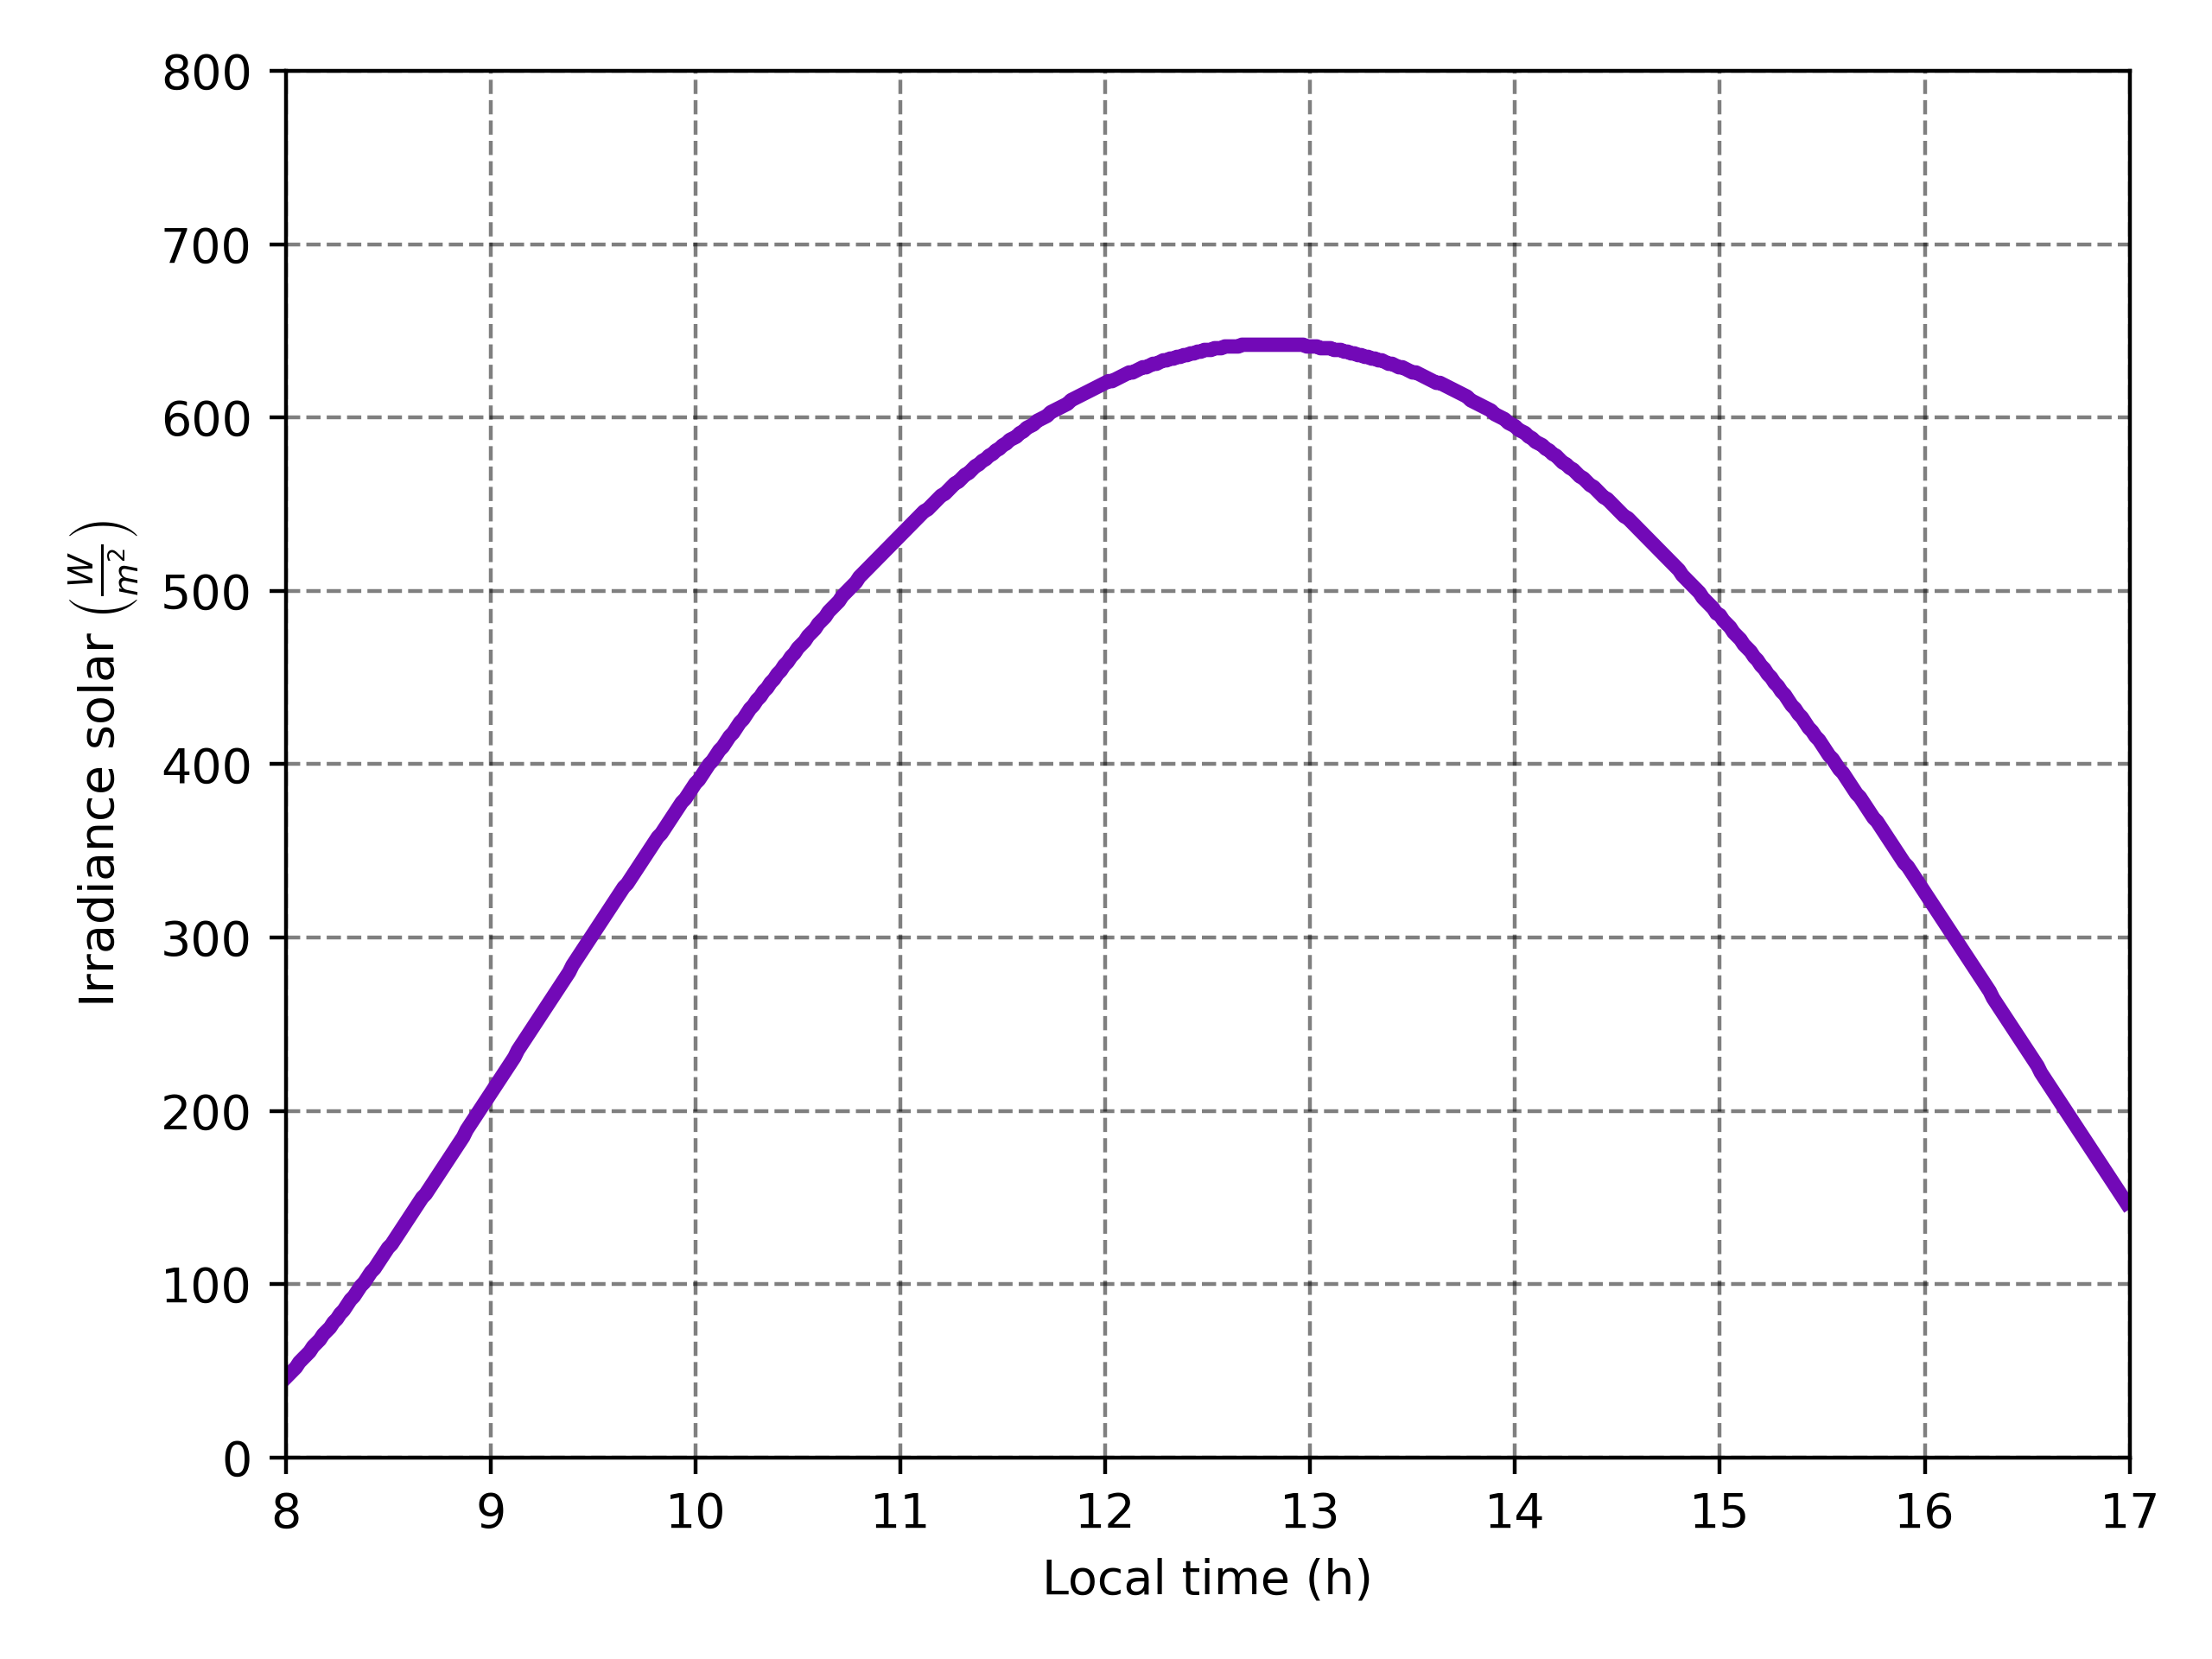
\includegraphics[width=6cm]{Irradiance.png}
        \end{figure}
    \end{minipage}
\end{frame}